% ============================================================================================
% This is a LaTeX template used for the course
%
%  I M A G E   B A S E D   B I O M E T R I C S
%
% Faculty of Computer and Information Science
% University of Ljubljana
% Slovenia, EU
%
% You can use this template for whatever reason you like.
% If you have any questions feel free to contact
% ziga.emersic@fri.uni-lj.si
% ============================================================================================

\documentclass[9pt]{IEEEtran}

% basic
\usepackage[english]{babel}
\usepackage{graphicx,epstopdf,fancyhdr,amsmath,amsthm,amssymb,url,array,textcomp,svg,listings,hyperref,xcolor,colortbl,float,gensymb,longtable,supertabular,multicol,placeins,minted}

 % `sumniki' in names
\usepackage[utf8x]{inputenc}

 % search and copy for `sumniki'
\usepackage[T1]{fontenc}
\usepackage{lmodern}
\input{glyphtounicode}
\pdfgentounicode=1

% tidy figures
\graphicspath{{./figures/}}
\DeclareGraphicsExtensions{.pdf,.png,.jpg,.eps}

% correct bad hyphenation here
\hyphenation{op-tical net-works semi-conduc-tor trig-gs}

% ============================================================================================

\title{\vspace{0ex} %
% TITLE IN HERE:
Structured data extraction from the Web
\\ \normalsize{Web Information Extraction and Retrieval 2018/19, Faculty of Computer and Information Science, University of Ljubljana}}
\author{ %
% AUTHOR IN HERE:
Matej Klemen, Andraž Povše, Jaka Stavanja
\vspace{-4.0ex}
}

% ============================================================================================

\begin{document}

\maketitle

\begin{abstract}
In this work we present our implementation of 2 different approaches for structured data extraction from the Web: using regular expressions and using XPath.
We test the implemented methods on 6 webpages from 3 different sources (Overstock, Rtvslo and Avto.net) and provide the outputs for the pages, generated by the methods.
\end{abstract}

\section{Introduction}

The Web is an ever-increasing collection of information. 
Probably the most used format for representing this information is HTML.
After crawling a webpage (which was done in the previous assignment) we would like to be able to automatically extract useful parts of the page.
Unfortunately, the popularity of HTML makes this task a little harder, since its primary goal is to make pages readable by humans, not necessarily computers.

For this assignment, we implement 2 different approaches to structured data extraction for 6 webpages from 3 different sources (Overstock, Rtvslo and Avto.net). 
These are data extraction using regular expressions and using XPath query language.

The rest of this report is structured as follows. 
In chapter \ref{section:used-data} we present the chosen 2 additional webpages, on which we test our methods.
In chapter \ref{section:methodology} we present the implementations of the 2 methods for structured data extraction and mention the obtained results.
In chapter \ref{section:conclusion} we conclude with a summary of what was done in this assignment.

\section{Used data}
\label{section:used-data}

In addition to the provided webpages from \textit{Overstock} and \textit{Rtvslo}, we select another source from which we obtain 2 similar webpages.
The third source on which we test our implemented methods are 2 webpages from \textit{Avto.net}. 
We made a query for two different vehicles, so we are dealing with lists of items.
The data items and data records we are interested in are shown in Figure\ref{fig:avtonet}.


\begin{figure}[h]
    \centering
    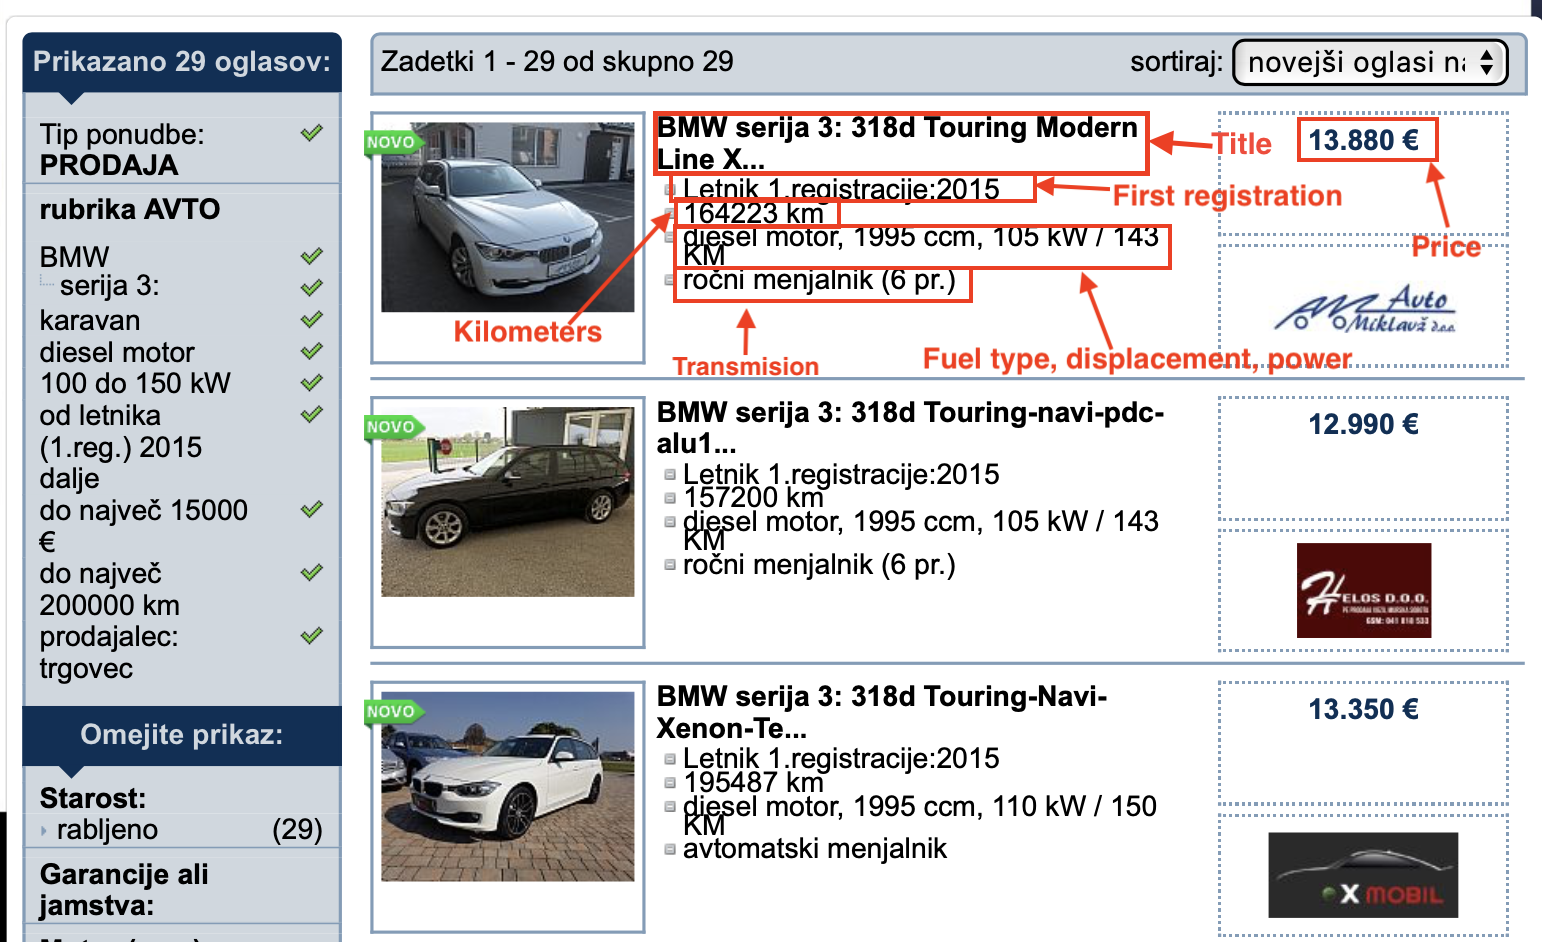
\includegraphics[width=1\columnwidth]{beemer.png}
    \caption{Selected website - AvtoNet and the data we are interested in extracting, outlined in red rectangles.}
    \label{fig:avtonet}
\end{figure}




\section{Methodology}
\label{section:methodology}

In this section we describe our implementations of the approaches using regular expressions and XPath query language.
The approach for extracting data from websites was split into two methods. One for the extraction of directly targeted elements that appear only once on the site (single items for the \textit{Rtvslo} website) and another for getting all results for elements that appear on a site multiple times (list items for the \textit{Overstock} website and \textit{Avto.net}). All the outputs that this extraction approach yields can be found in the git repository (in the folder \verb/output\regex\/, where each website has it's own JSON file).

\subsection{Approach using regular expressions}
\label{section:regex}

\subsubsection{Single items}
The regular expressions for extracting single elements were written in such a way that they start to capture text when they encounter the targeted html element, which wraps the data that we wish to extract. To search for the exact element, we look at the HTML source of the webpage and find the tag and it's classes and attributes to refine the search pattern. For example, if we were searching for data inside the \mintinline{HTML}{<div class="author-name">Miha Merljak</div>} element, the regular expression would look like \verb/<div class=\"author-name\">(.*)<\/div>/. Here, we start by searching for the div element with the class \textit{author-name} and we create a capture group for all the characters that are there until we reach the closing tag. All of the other elements on this page were retrieved in a similar fashion, except for the elements whose tags didn't feature such a specific tag. In that case, we looked for their parent elements, that we could target and then skipped all characters, until we reached our desired nested tag, from which we then captured the text. That was done using an expression such as~\verb/<header class=\"parent\">[\S\s]*?<h1>(.*)<\/h1>/, where \verb/[\S\s]*?/ ignores all the characters (if there are any) until we reach our nested h1 tag. We find the first element that is captured by the regular expression on the input website, extract the text and send it into serialization. This approach was used for the Rtvslo elements' text retrieval.

\subsubsection{List items}

This approach works in a similar way as the one for extracting single items, where we use HTML tags and their specific attributes to target certain elements of the webpage. The difference here was that instead of finding the first element only, we captured all the elements that our regular expression found on the input website that matched against it and created a list of all such items.
The idea is to find all names, prices, descriptions and similar properties of items and then take each match (there is the same amount of matches for each item) and map it together into an object for each item, listed on the webpage.

For example, if there are two items, that have a name and a price on the website, we first extract all the names and then all the prices. Next, we combine the first name with the first price, etc. To handle missing items for each element, the failsafe was constructed with the \textit{or} operator inside the capture group. In the case of parsing prices of cars on the \textit{Avto.net} page, we can encounter a price or a ''Pokličite za ceno'' element. For that specific case, we construct a regular expression, that contains a capture group like \verb/([^\t\n>]*?€|Pokličite za ceno!)/, which can either extract a price in Euros or the text ''Pokličite za ceno''. We later map ''Pokličite za ceno'' into \mintinline{python}{None} in Python to ensure a more international and flexible object output.

\subsection{Approach using XPath}
\label{section:XPath}
\subsubsection{RTVSlo}
We first approached extracting elements from RTVSlo website. The methods used to get single items and later a list of all items were used in the same manner as stated above in the Regex subsection\ref{section:regex}. The locations of author, content and other items, was quite well defined within the webpage. Items had their unique class and perhaps some other HTML element, like "h1". We wanted to extract text, so we used the text() function in XPath. An example of such XPath query for the content is 
\verb|"//*[@class=\"Body\"]/text()"|.
\subsubsection{Overstock}
Overstock website proved to be built quite differently and was extracted using a different approach. 
The entire approach of the HTML structure is a bit outdated and everything is structured using multiple nested tables and such not very friendly for building an XPath query per se. 
The query was then built by essentially traversing the tables, till we reached our desired element. 
Because the wanted elements, are near each other, we could reuse the base location of each item and build the query on top of that. 
An example query for extracting the title, with base location included as query
\begin{verbatim}
"/html/body/table/tbody/tr/td[5]/table/tbody/tr/td/
table/tbody/tr/td/table/tbody/tr/td/a/b/text()"
\end{verbatim}

\subsubsection{AvtoNet}
Last website we extracted using XPath was avtonet. It proved to be a mixture of the two approaches we used above. The kind of base location for all elements we wanted to retrieve was reachable using the unique class identifier, whereas specifics required a traversal of the table. 
Because of that, we used simillar approach as with Overstock, by reusing the base location of elements.
There were also some elements, within the same HTML tags divided by a comma, so we had to split them manually using Python.
These elements were Fuel type, Displacement and Power, and were split using the Python \verb/split(',')/ function. 
There was also a problem, that some items did not have all the elements. In a case, where there were no Kilometers provided, we have to deal with an IndexError, which we caught and handled successfully. 
An example of an XPath query for extracting transmission information
\begin{verbatim}
"//*[@class=\"ResultsAdDataTop\"]/ul/li[4]/text()"
\end{verbatim}

\subsection{Data serialization}
After the data has been extracted using different methods, there were still some unicode newline and tab characters left in the texts. We ran a simple \mintinline{python}{strip()} function call on the strings to filter them out.
However due to the limit that all the data needs to be extracted will regular expressions only, we were still unable to filter some of the noisy symbols out in some cases.

When we assembled our data objects (Python dictionaries or lists) with the data extracted from webpages, the output was then serialized into a JSON object using Python's in-built \verb/json/ module.

\section{Conclusion}
\label{section:conclusion}
We presented 2 approaches to structured data extraction from the Web: using regular expressions and using XPath query language.
We applied these methods to 6 webpages and provided the methods' output.
The third, more general, approach to structured data extraction (using RoadRunner algorithm) was sadly not implemented.


\end{document}